\documentclass[14pt]{beamer}
%\documentclass[handout]{beamer} %Makes Handouts
%\usetheme{Singapore} %Gray with fade at top
\useoutertheme[subsection=false]{miniframes} %Supppress subsection in header
\useinnertheme{rectangles} %Itemize/Enumerate boxes
\usecolortheme{seagull} %Color theme
\usecolortheme{rose} %Inner color theme

\definecolor{light-gray}{gray}{0.75}
\definecolor{dark-gray}{gray}{0.55}
\setbeamercolor{item}{fg=light-gray}
\setbeamercolor{enumerate item}{fg=dark-gray}

\setbeamertemplate{navigation symbols}{}
%\setbeamertemplate{mini frames}[default]
%\setbeamercovered{dynamics}
\setbeamerfont*{title}{size=\Large,series=\bfseries}

\setbeamertemplate{frametitle}{\vspace{.5em}\bfseries\insertframetitle}
\newcommand{\heading}[1]{\noindent \textbf{#1}\\ \vspace{1em}}

% small footnotes
\setbeamerfont{footnote}{size=\tiny}

\usepackage{bbding,color,multirow,ccaption,tabularx,graphicx,verbatim}
\usepackage[english]{babel}
\usepackage[latin1]{inputenc}
\usepackage[T1]{fontenc}
\usepackage{lmodern}
\usepackage{alltt}

\usepackage{pdfpages}
\usepackage{tikz}
\usetikzlibrary{positioning} 
\usetikzlibrary{trees}


\setbeamertemplate{background}{
\includegraphics[width=\paperwidth,height=1.05\paperheight,keepaspectratio]{images/lse2.png}}
%\setbeamertemplate{footline}[frame number]

\title{Reproducibility with\\git and rmarkdown}
\author[]{Thomas J. Leeper}
\institute[]{
  \inst{}%
  Department of Government\\London School of Economics and Political Science
}

\date[]{30 January 2018}

\begin{document}

\frame{\titlepage}

% http://swcarpentry.github.io/git-novice/
% https://www.atlassian.com/git/tutorials/comparing-workflows#!workflow-gitflow


\section{Background}


\frame{

\frametitle{Version Control as Organization}
	
	\begin{itemize}\itemsep1em
	\item Version control helps you stay organized
		\begin{enumerate}
		\item<2-> What's important to keep around?
		\item<3-> What's not important to keep around?
		\item<4-> What is all this crap?
		\end{enumerate}
	\item<5-> Think ``tracked changes'' for all of your files
		\begin{itemize}
		\item<6-> Save history of changes/versions
		\item<7-> Experiment non-destructively
		\item<8-> Collaborate
		\end{itemize}
	\item<9-> You're probably already version controlling informally!
	\end{itemize}

}

\frame{

\only<1>{
\includegraphics[width=\textwidth]{images/phd1531-1}}

\only<2>{
\includegraphics[width=\textwidth]{images/phd1531-2}}

\only<3>{
\includegraphics[width=\textwidth]{images/phd1531-3}}

}


\frame{
\begin{center}

\includegraphics[height=\textheight]{images/prospectus}
\end{center}
}


\frame{

\frametitle{Wait, but why do we care?}

If we're going to be transparent \textit{in the end} (e.g., at replication or data archiving stage), what do we need to provide?

\begin{itemize}\itemsep1em
\item<2-> A well-organized, reproducible analysis!
\end{itemize}

\only<3->{So rather than make that an annoying, post-hoc exercise related to publication, try to get organized and stay organized throughout your project from the very beginning.}

}

\frame{


\includegraphics[width=\textwidth]{images/nextweek}

}


\section{Git}


\frame{
\frametitle{Git}

\begin{itemize}\itemsep1em
\item Git is ``an open-source distributed version control system''
\item Developed in 2005 by Linus Torvalds
\item Widely used in software development world
\end{itemize}

}

\frame{

\frametitle{Why use Git for open science?}

\begin{itemize}\itemsep1em
\item<2-> Helps you keep and \textit{annotate} snapshots of your project over time
	\begin{itemize}
	\item Better than renaming your files all the time
	\item Better than using within-file VCS (e.g., Word)
	\item Better than single-stream sharing (e.g., Dropbox)
	\end{itemize}
\item<3-> Facilitates collaboration (incl. with future you)
\item<4-> It's FOSS with lots of clients, tools, and community support
	\begin{itemize}\itemsep1em
	\item Widely used in software development world
	\end{itemize}
\end{itemize}


}


\frame{

\frametitle{Using Git}

\begin{itemize}\itemsep1em
\item Git create a ``local repository'' file that you can interact with using a number of tools
	\begin{itemize}
	\item Command-line \texttt{git}
	\item Git Bash
	\item Git GUI
	\item GitHub Desktop
	\item RStudio (via ``Projects'')
	\item GitHub/Bitbucket/GitLab web interfaces
	\item Gitkraken
	\item git2r (R package)
	\item \dots
	\end{itemize}
\end{itemize}

}

\frame<1-7>[label=essentials]{

\frametitle{Git Essentials}

\begin{enumerate}\itemsep0.5em
\item \texttt{stage}
	\only<2>{
	\begin{itemize}
	\item \textbf{stage}: select files to be recorded in a ``snapshot'' of the project
	\item \textbf{unstage}: remove files from the snapshot (but not from your computer)
	\end{itemize}
	}
\item \texttt{commit}
	\only<3>{
	\begin{itemize}
	\item \textbf{commit}: record a permanent snapshot of the staged files, labelled with a ``commit message''
	\item \textbf{amend}: modify (typically the most recent) commit with new changes or commit message
	\end{itemize}
	}
\item \texttt{branch}
	\only<4>{
	\begin{itemize}
	\item produce a complete \textit{local} copy of the project where changes can be made independently of the ``master'' branch
	\end{itemize}
	}
\item \texttt{merge}
	\only<5>{
	\begin{itemize}
	\item update a branch with changes from another local branch (or a remote); you can change multiple branches independently.
	\end{itemize}
	}
\item \texttt{push} and \texttt{pull}
	\only<6>{
	\begin{itemize}
	\item \textbf{push}: send the project (any new commits) to a remote server (like GitHub)
	\item \textbf{pull}: grab new commits from a remote server
	\end{itemize}
	}
\end{enumerate}


}


\frame{
\vspace{2em}
{\LARGE \textbf{Hands-on practice!}}
}


\frame{

\small

\begin{alltt}
git -{}-version

git

git config -{}-global user.name "My Name"

git config -{}-global user.email "me@example.com"

git config -{}-list

\end{alltt}
}


\frame{
\begin{alltt}
git init

git status

echo Hello world! > README.md

git add README.md

git status

git rm -{}-cached README.md

git status

git add -{}-all

git commit -m "my first commit!"

git status
\end{alltt}
}


\frame{

\frametitle{Initializing a Project Structure}

\begin{itemize}\itemsep1em
\item There's no single best way to organize a project
\item But, some words of wisdom:
	\begin{itemize}
	\item Put like with like
	\item Avoid excessive hierarchy
	\item Not everything needs to go into git
	\item Steal others' structures!
	\end{itemize}
\end{itemize}

}

\frame<1>[label=ideal]{
    \frametitle{What makes up the ideal reproducible research product?}
    
   	\begin{itemize}\itemsep0.5em
   	\item Gandrud's template
   	\item rOpenSci's ``Research Compendium''
   	\item Project TIER
   	\end{itemize}
    
}

\frame[label=gandrud]{
%%%%%%%%%%%%%%
% Example research project file path
% Christopher Gandrud
% Updated 21 October 2014
%%%%%%%%%%%%%%

% Set node styles
\tikzstyle{DirBox} = [draw=black,
                      rectangle,
                      minimum width=4em,
                      very thick,
                      font=\tiny]

\tikzstyle{every node} = [draw=gray,
                          thin,
                          anchor=west,
                          font=\tiny]

% Begin tikz picture
\begin{tikzpicture}[scale=0.9,%
  grow via three points={one child at (0.5,-0.7) and
  two children at (0.5,-0.7) and (0.5,-1.4)},
  edge from parent path={(\tikzparentnode.south) |- (\tikzchildnode.west)}]
  % Root Directory
  \node (root) at (5, 10) [DirBox]{Root};

  % Project Directory
  \node (project) at (4.425, 9) [DirBox]{Rep-Res-ExampleProject1}
        child {node {{\tiny{Paper.Rnw}}}}
        child {node {{\tiny{Slideshow.Rnw}}}}
        child {node {{\tiny{Website.Rnw}}}}
        child {node {{\tiny{Main.bib}}}}
            ;

  % Data Directory
  \node (data) at (0, 6.5) [DirBox]{Data}
      child {node {{\tiny{MainData.csv}}}}
      child {node {{\tiny{Makefile}}}}
      child {node {{\tiny{MergeData.R}}}}
      child {node {{\tiny{Gather1.R}}}}
      child {node {{\tiny{MainData\_VariableDescriptions.md}}}}
      child {node {{\tiny{README.Rmd}}}}
        ;

  % Analysis subdirectores/files
  \node (analysis) at (1.5, 8) [DirBox]{Analysis}
      child {node {{\tiny{GoogleVisMap.R}}}}
      child {node {{\tiny{ScatterUDSFert.R}}}}
        ;

  % README file
  \node (readme) at (9.5, 7) {README.md};

  % Connect boxes that are not explicit children
  \draw (root) -- (project);
  \draw (project) -| (analysis);
  \draw (analysis) -| (data);
  \draw (project) -| (readme);

\end{tikzpicture}
}


\begin{frame}[fragile, label=package]

\footnotesize

\begin{verbatim}
project
|- DESCRIPTION      # project metadata and dependencies 
|- README.md        # top-level description of content
|
|- data/            # raw data, not changed once created
|  +- my_data.csv   # data files in open formats
|
|- analysis/        # any programmatic code 
|  +- my_scripts.R  # R code used to analyse data 
\end{verbatim}

\end{frame}

\frame[label=tier]{
    \begin{center}
        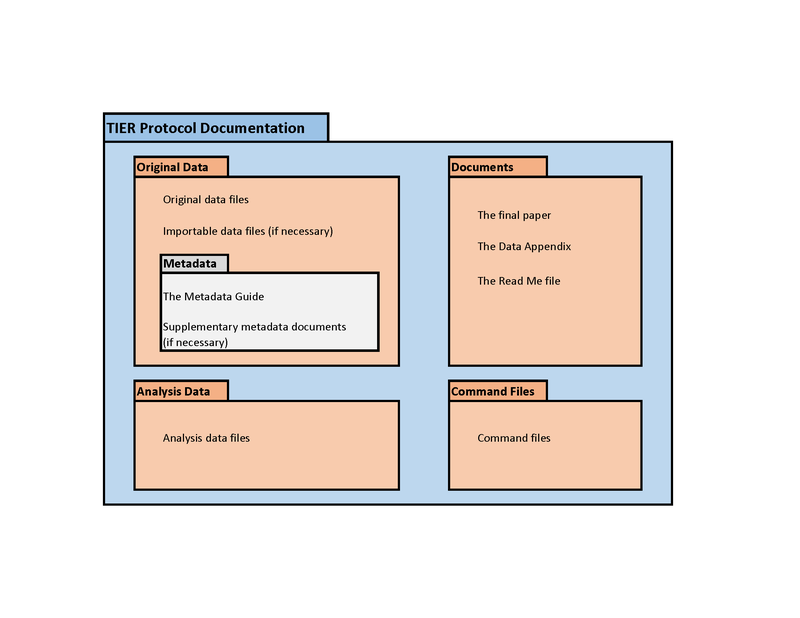
\includegraphics[width=\textwidth]{images/project-tier}
    \end{center}
}

\frame{

\includegraphics[width=\textwidth]{images/badfolder}
}

% structure

\frame{
\begin{alltt}
mkdir code

mkdir data

mkdir figures

git status
\end{alltt}
}

\frame{
\begin{alltt}
git status

cat README.md

\# do something to README.md

git diff

git add README.md

git commit -m "second commit"

git status

git log

git log -{}-oneline

git log -{}-oneline -1

git log -{}-oneline -{}-stat
\end{alltt}
}



\frame{}


\section{Intermediate Git}

\frame{
\begin{alltt}
git status

git diff README.md

git diff HEAD README.md

git diff HEAD\textasciitilde1 README.md

git diff HEAD\textasciitilde2 README.md

git diff HEAD\textasciitilde3 README.md

git diff HEAD\textasciitilde20 README.md

git diff <commit hash> README.md

git diff <commit hash>
\end{alltt}
}


\frame{

\frametitle{!! DANGER: Amend Commit !!}
\begin{alltt}
git status

git log -{}-oneline

\# maybe add/rm files

git amend

\# enter the hell of vim

\vspace{1em}

git config -{}-global core.editor\\ "<executable> <options>"
\end{alltt}
}


\frame{

\frametitle{Safe reversion}
\begin{alltt}
git status

git log -{}-oneline

git revert <commit hash>

\# enter the hell of vim

\# or something else terrible

git revert -{}-abort
\end{alltt}
}

\frame{

\frametitle{!! DANGER: Unsafe reversion !!}

\href{https://stackoverflow.com/questions/927358/how-to-undo-the-last-commits-in-git}{\textit{The} StackOverflow Question}
}



% ignoring things
\frame{
\begin{alltt}
git status

echo "bad bad bad" > bad.txt

git status

echo bad.txt > .gitignore

git status

echo bad bad bad > bad1.txt

echo bad bad bad > bad2.txt

echo bad* > .gitignore

git status

git add bad1.txt -f

git status
\end{alltt}
}


% going back in history
\frame{
\frametitle{Navigating History}

\begin{alltt}
git status

git log

git checkout <commit hash>

git status

ls

cat README.md

git checkout master
\end{alltt}
}


% changing history
\frame{
\begin{alltt}
git status

git log

git checkout <commit hash>

git status

ls

echo aaaaaah!>manuscript.txt

git checkout master
\end{alltt}
}


\frame{

\begin{center}
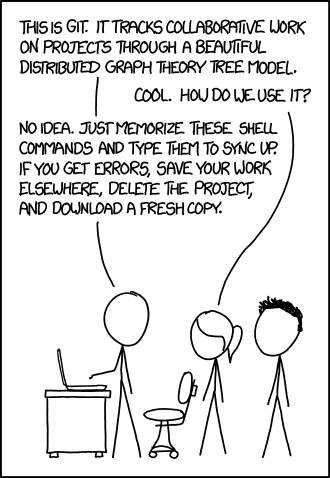
\includegraphics[height=\textheight]{images/xkcd1597}
\end{center}

}


\frame{}

\section{Branches \& Remotes}

\frame{
\frametitle{Branches}
\begin{itemize}\itemsep1em
\item Branches are local, parallel versions of your entire project
\item Useful for multiple things:
	\begin{itemize}
	\item Experimentation
	\item Manuscript submissions
	\item Collaboration
	\end{itemize}
\end{itemize}
}


\frame{
\begin{center}
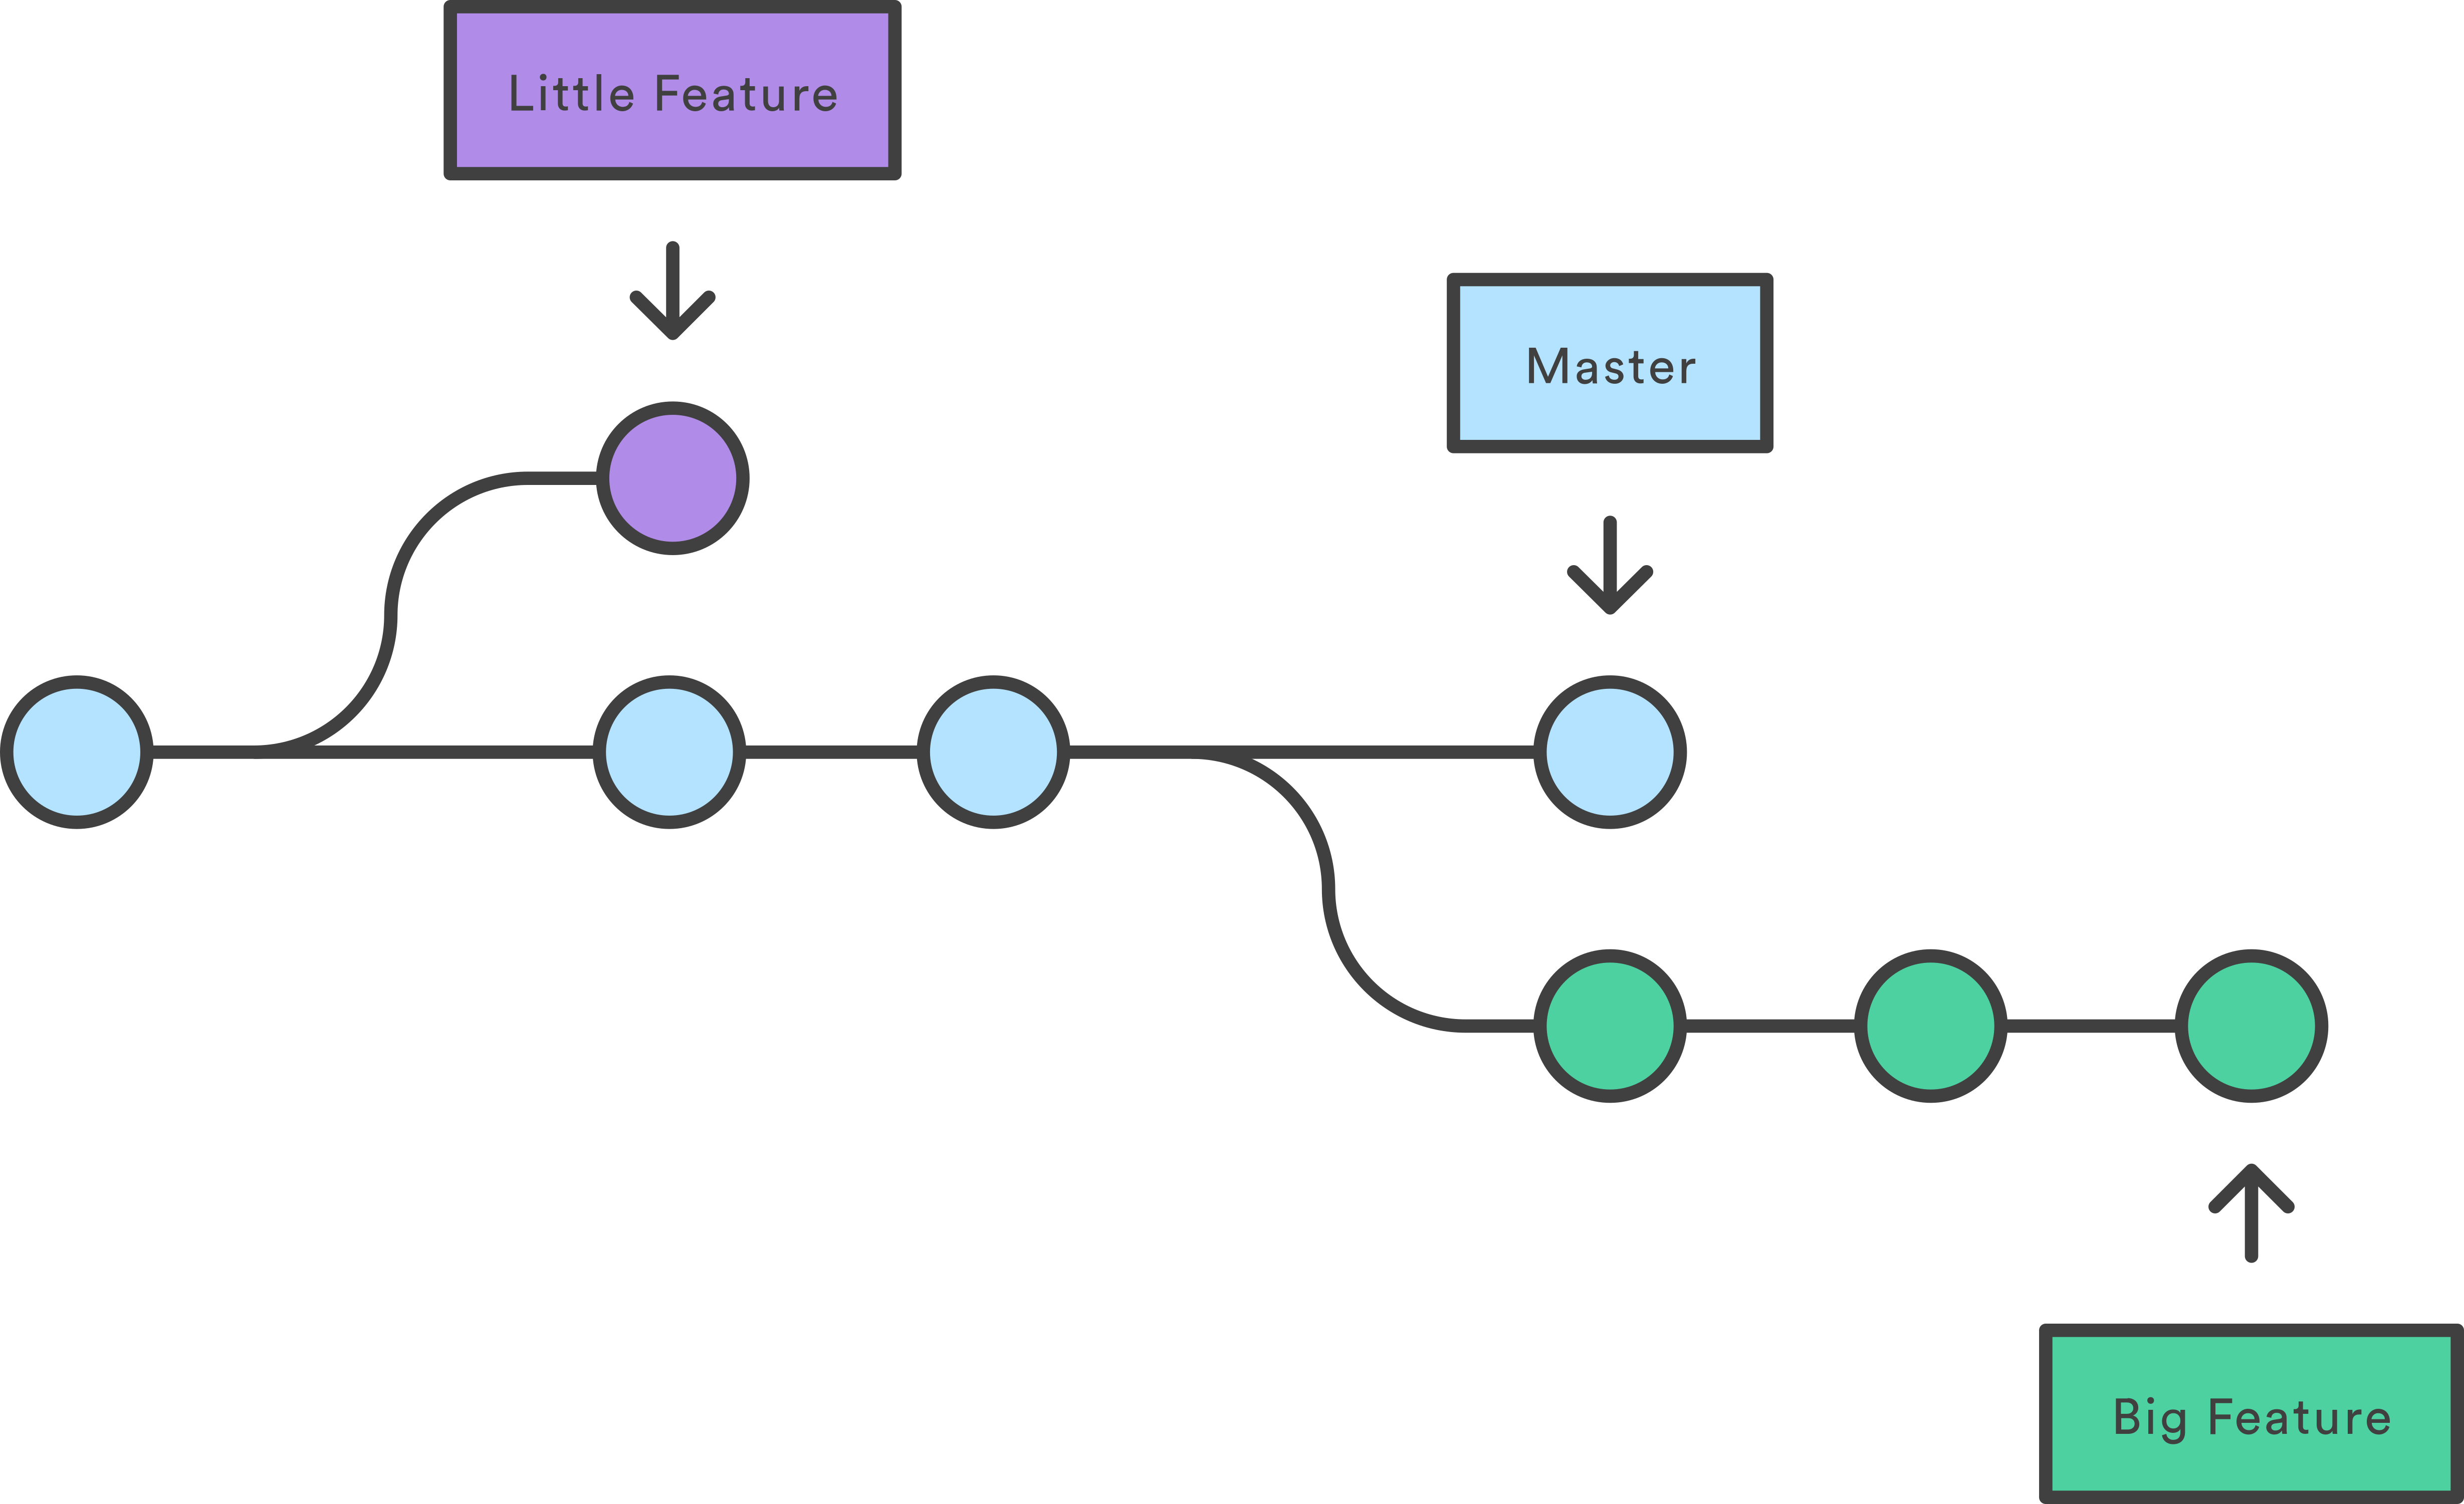
\includegraphics[width=\textwidth]{images/atlassian-branching}
\end{center}

\footnotesize{Source: \url{https://www.atlassian.com/git/tutorials}}
}


\frame{
\begin{center}
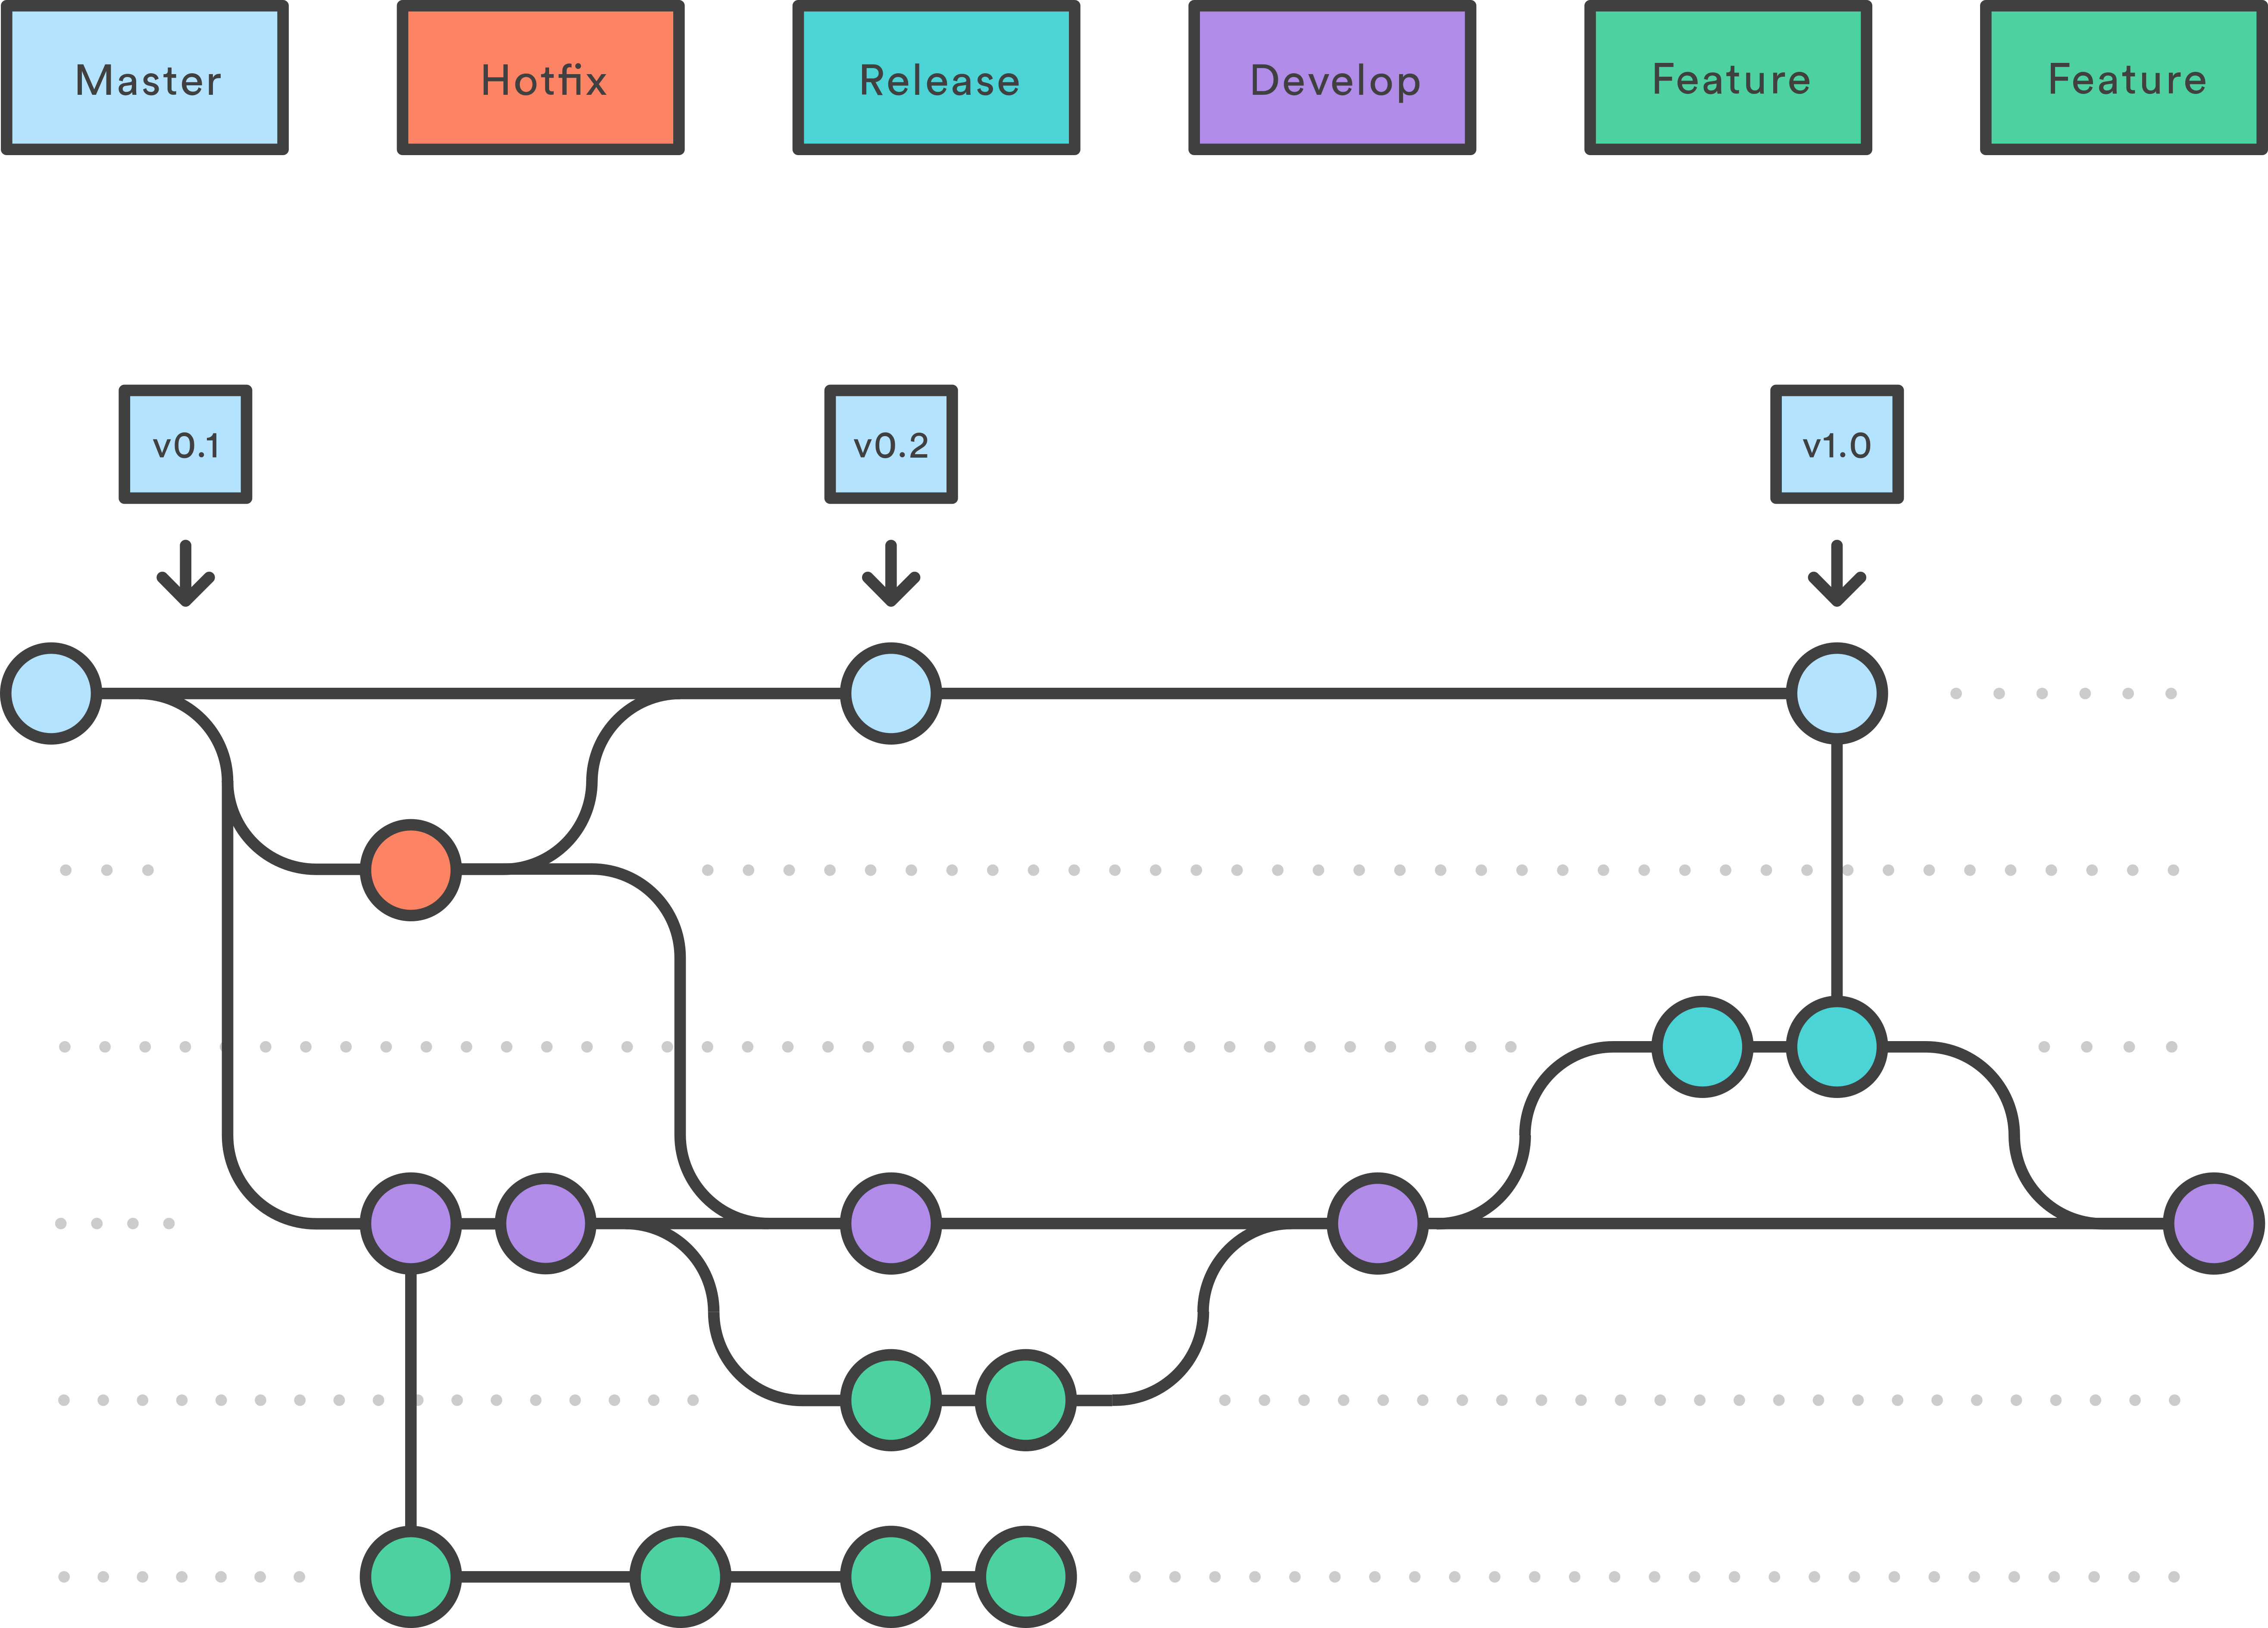
\includegraphics[height=.75\textheight]{images/atlassian-branching-2}
\end{center}

\footnotesize{Source: \url{https://www.atlassian.com/git/tutorials}}
}


\frame{
\frametitle{Simple branch and merge}
\begin{alltt}
git status

git checkout -b thomas

git status

\# do something

git add -{}-all

git commit -m "thomas's commit"

git checkout master

git branch

git log -{}-graph -{}-oneline

git merge thomas
\end{alltt}
}


% GUIs
\frame{
\frametitle{GUIs}

\begin{itemize}\itemsep1em
\item You can do everything in Git on the command line

\item GUIs can be helpful for:

	\begin{itemize}\itemsep0.5em
	\item Exploring history
	\item Visualizing branches
	\item Confirming what you're doing
	\end{itemize}
\end{itemize}

}




\frame{
\frametitle{Merge conflicts}
\begin{alltt}
git checkout -b thomas

git status

\# do something to README.md

git add -{}-all

git commit -m "change on thomas"

git checkout master

\# do something to README.md

git add -{}-all

git commit -m "change on master"

git merge thomas

git log
\end{alltt}
}


\frame{}



\frame{
\frametitle{Remotes}
\begin{itemize}\itemsep1em
\item A server (``cloud'') instance of the Git repository
\item Useful for multiple things:
	\begin{itemize}
	\item Collaboration
	\item Transparency
	\item Archiving/backups
	\item Using web-based Git interfaces
	\end{itemize}
\end{itemize}
}

\frame{
\frametitle{Remotes}
\begin{itemize}\itemsep1em
\item Three major players in cloud Git
	\begin{itemize}
	\item GitHub
	\item Atlassian Bitbucket
	\item GitLab
	\end{itemize}
\item Why choose one or the other?
	\begin{itemize}
	\item Cost
	\item Collaborators
	\item Private repositories
	\end{itemize}
\end{itemize}
}


\frame{
\begin{alltt}
git status

git remote add github\\ https://github.com/leeper/rt2

git remote

git remote set-url

git remote rename

git remote remove
\end{alltt}
}
	

\frame{
\begin{alltt}
git status

git push github master -u

git fetch github

git fetch github master

git checkout -b new-idea

git push github new-idea

git checkout master

git pull github master

git pull
\end{alltt}
}


\frame{}

\frame{
\begin{alltt}
git status

git tag -a v0.0.1 -m "v0.0.1"

git push -{}-tags


git tag -d v0.0.1
\end{alltt}
}


\frame{

\frametitle{Tags versus Branches}

\begin{itemize}\itemsep1em
\item \textit{Branches} are for working versions of project

	\begin{itemize}
	\item Collaborator-specific branches
	\item Submission-specific branches
	\item Experimental or ``bug fix'' branches
	\end{itemize}

\item \textit{Tags} are for marking particular snapshots

	\begin{itemize}
	\item Significant moments in project history
	\item Journal submission or conference version
	\item Formal ``releases''
	\end{itemize}

\end{itemize}

}


% collaborating

\frame{
\frametitle{Collaboration}

\begin{itemize}\itemsep2em
\item Technical aspects
	\begin{itemize}
	\item Give collaborators access on GitHub (or wherever)
	\item Work on separate branches
	\item Merge agreed changes into \textbf{master}
	\end{itemize}

\item Human factors aspects
	\begin{itemize}
	\item Requires agreeing on workflow
	\item Communication about what goes in ``master''
	\item Can feel awkward if moving from a Dropbox- or email-based collaboration style
	\end{itemize}
\end{itemize}

}


% merging collaborators

\frame{
\frametitle{Try it with a partner!}
\small
\begin{enumerate}\itemsep0.5em
\item Partner A create a GitHub repo; give Partner B access
\item Partner B should \texttt{git fetch}/\texttt{git pull} the repo
\item Partner B should create a local branch and \texttt{git push}
\item Partner A should \texttt{git fetch} the branch
\item Partner A should \texttt{git merge} the branch to \textbf{master} and \texttt{git push}
\item Partner B should \texttt{git pull} from \textbf{master}
\item Both use \texttt{git log} to compare
\end{enumerate}
}


\frame{}


\frame{

\frametitle{Conclusion}

\begin{itemize}\itemsep1em
\item Once you use Git, you'll never want to go back to your old workflow
\item<2-> But, collaborators probably don't know or want to use Git!
\item<3-> Git is crazy complicated -{}-- StackOverflow is your friend
\end{itemize}

}

\frame{}

\appendix

\section{Dynamics Documents in R}

\frame{}

\frame{
\Large
\begin{center}
How do you typically get figures, tables, and other material out of analytic software and into papers or presentations?
\end{center}
}


\frame{
\frametitle{Dynamic Documents in R}
\begin{itemize}\itemsep1em
\item The dynamic documents landscape is evolving very, very rapidly:
	\begin{itemize}
	\item Early 2000s: Sweave
	\item 2010's: knitr
	\item Ongoing: Rmarkdown
	\end{itemize}
\item<2-> Embed code (R or otherwise) inside a manuscript that outputs:
	\begin{itemize}
	\item Word (.docx)
	\item HTML
	\item LaTeX/PDF
	\item HTML or PPT slides
	\end{itemize}
\end{itemize}
}

\frame{
\begin{alltt}
\# My Manuscript

Thomas J. Leeper

This is my manuscript.
\end{alltt}
}


\begin{frame}[fragile]

\frametitle{Rmarkdown}

\begin{enumerate}\itemsep0.5em
\item YAML metadata header
\item Document contents in \textbf{markdown}
\item Code in ``code chunks'':

\begin{verbatim}
```{r chunk1}
# R code
hist(rnorm(1000))
```
\end{verbatim}
\end{enumerate}

\end{frame}


\begin{frame}[fragile]
\begin{verbatim}
---
- title: My Manuscript
- author: Thomas J. Leeper
- date: 2017-09-21
- output: pdf_document
---

This is my manuscript.

```{r chunk1}
# R code
hist(rnorm(1000))
```
\end{verbatim}
\end{frame}


\frame{

\frametitle{Markdown Basics}

Markdown is a very simple markup language for formatting simple texts:\\

\vspace{1em}

\begin{tabular}{ll}
\texttt{*italics*} & \textit{italics} \\
\texttt{*bold*} & \textbf{bold} \\
\texttt{`preformatted`} & \texttt{preformatted} \\
\texttt{\# Heading} & Heading Level 1 \\
\texttt{\#\# Heading} & Heading Level 2 \\
\texttt{\#\#\# Heading} & Heading Level 3 \\
\texttt{[link](https://google.com)} & \href{https://google.com}{link} \\
\end{tabular}

}

\frame{}



\begin{frame}[fragile]

\frametitle{Chunk Options}

\begin{verbatim}
```{r chunk1, eval=TRUE, echo=TRUE}
2 + 2
```

```{r chunk2, eval=TRUE, echo=FALSE}
2 + 2
```

```{r chunk3, echo=FALSE, results="hide"}
2 + 2
```
\end{verbatim}
\end{frame}


\begin{frame}[fragile]

\frametitle{Global Chunk Options}

\begin{verbatim}
```{r options, eval = TRUE, echo = FALSE}
library("knitr")
opts_chunk$set(echo = FALSE, 
               cache = TRUE, 
               message = FALSE)
```
\end{verbatim}
\end{frame}


\begin{frame}[fragile]
\frametitle{Basic Tables}

\small

\begin{verbatim}
```{r table1, results = "asis"}
xtable::xtable(table(mtcars$cyl, mtcars$gear))

knitr::kable(head(mtcars))
```
\end{verbatim}
\end{frame}


\begin{frame}[fragile]
\frametitle{Regression Results Tables}
\begin{verbatim}
```{r table2, results = "asis"}
library("stargazer")
stargazer(
  x1 <- lm(mpg ~ disp + wt, 
           data = mtcars),
  x2 <- lm(mpg ~ disp + wt + vs, 
           data = mtcars),
  header = FALSE
)
```
\end{verbatim}
\end{frame}


\begin{frame}[fragile]
\frametitle{Figures}	
\begin{verbatim}
```{r fig1, 
    fig.cap = "Fuel Economy by Weight",
    fig.height = 4,
    fig.width = 6}
library("ggplot2")
ggplot(mtcars, 
    aes(x = wt, 
        y = mpg,
        colour = factor(cyl))) + 
  geom_point()
```
\end{verbatim}
\end{frame}



\end{document}
